\chapter{Current Implementation}
\label{chapter:myImplementation}

Since the idea of main concept for the current implementation is based on trees, more specifically quad trees, we present the relevant general ideas of tree at first and explain how they are related to this implementation. The theory presented in this section is based on a book by Goodrich et al. unless otherwise stated\cite{goodrich2007data}.

 \section{General ideas about tree structure}
 
 		
		Productivity experts claim that breakthroughs come by thinking "nonlinearly". Tree structures have been an enormous leap in data organization since they allow the implementation of algorithms more rapidly than linear data structures such as lists, vectors and sequences. 
		
		In categorizing trees as "nonlinear" with respect to organizational relationship, the main feature that must be highlighted is more sophisticated relationships than elementary "before" and "after" relationships between objects in sequences. A tree follows a \textbf{hierarchical} architecture, with some objects being "above" and some "below" others. 
		
		A \textbf{tree} is an abstract data type. In a tree, each element has a \textbf{parent} element. It can have zero or more \textbf{children} elements.
		\\
		\textbf{Formal Tree Definition}
		
		A \textbf{tree T} can be defined as a set of \textbf{nodes} storing elements in a \textbf{parent-child} relationship and has the properties as defined below:
		\begin{itemize}
			\item A nonempty \textbf{T} has a special node known as the \textbf{root} of \textbf{T} which has no parent. 
			\item Every other node \textit{$\nu$} of \textbf{T} has a unique parent node \textit{w} and every node with parent \textit{w} is a \textbf{child} of \textit{w}.
		\end{itemize}

		If a parent has two nodes which are its children, then these children are \textbf{siblings}. If a node \textit{$\nu$} does not have children then it is \textbf{external} while it is \textbf{internal} if it has one or more children. External nodes can also be termed as \textbf{leaves}.
		
		Figure \ref{fig:GeneralTree} shows an example of a tree representing computer files organized in the form of nested directories. 
		
		\begin{figure}[h]
			\centering
			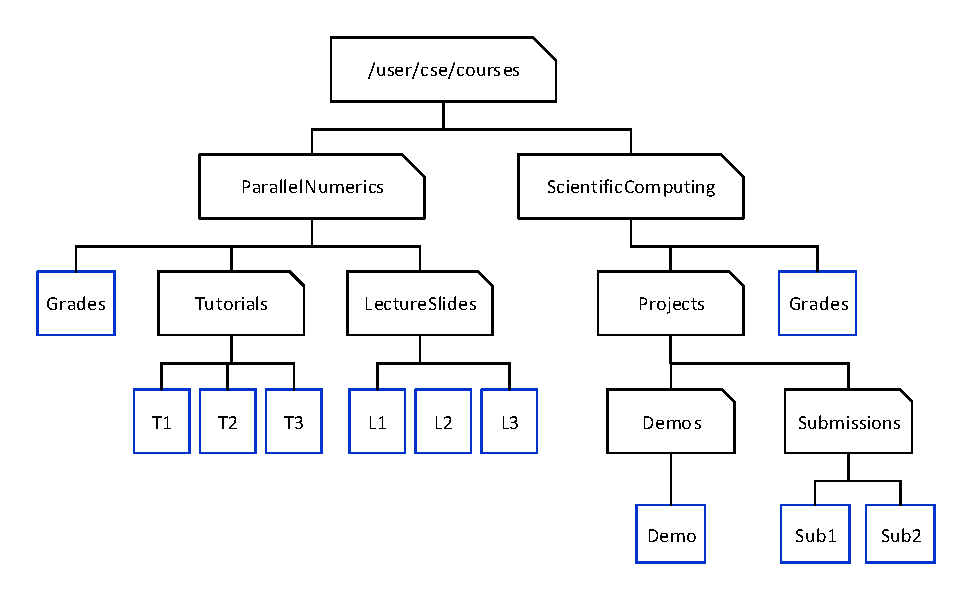
\includegraphics[width=\textwidth]{/GeneralTree.pdf}
			\caption{Tree representing a portion of a file system}
			\label{fig:GeneralTree}
		\end{figure}
		The relation of this to our implementation is that the external nodes are the nodes which doesn't require more refining.
		\textbf{Ordered Trees}
		
		A tree having a linear ordering for the children of each node is termed as \textbf{ordered}. The children of a node can be identified as first, second and so on. In ordered trees, linear order relationship between siblings is illustrated by listing them in a sequence.
		
		For implementation purposes "position" and "node" can be used interchangeably for trees. \\
		
		Later it can be observed how the nodes are exactly a full grid solution or projection of combination technique solution on to full grid one.\\
		\textbf{A Linked Structure for General Trees}
		
		A \textbf{linked structure} can be used to comprehend a tree \textbf{T}. Each node of \textbf{T} can be depicted as a position object \textit{p} with the below mentioned fields:
		reference to the node's element, link to node's parent and some kind of collection to store links into node's children.  Figure \ref{fig:LinkedStrucGenTree} shows a representation of  a node of a tree and a schematic representation of the data structure associated with a node and its children. \\
		
		% The height of a tree is equal to the maximum depth of its external nodes.
		\begin{figure}[h]
			\centering
		    \begin{subfigure}[b]{0.33\textwidth}
			    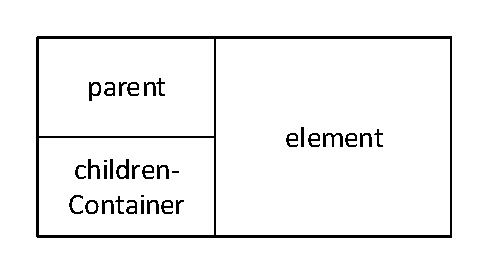
\includegraphics[width =\textwidth]{/LinkedStrucGenTree1.pdf}
			    %\vspace{3em}
				\centering
		        \caption{}
		    \end{subfigure} 
		    \begin{subfigure}[b]{0.66\textwidth}    
			    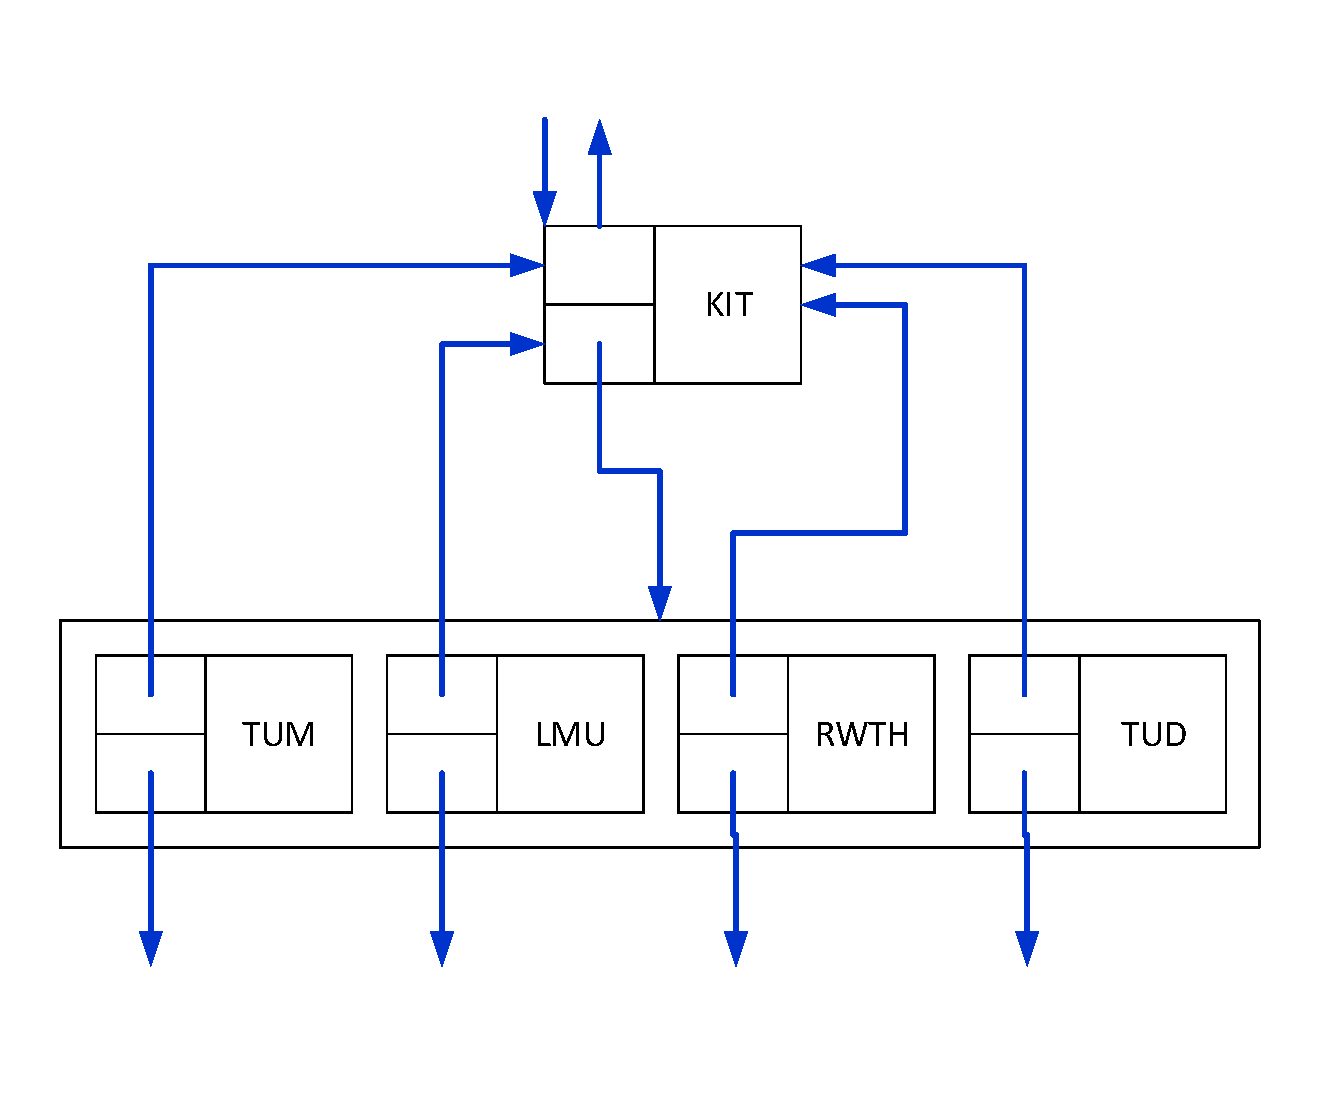
\includegraphics[width =\textwidth]{/LinkedStrucGenTree2.pdf}
				\centering    
			 \caption{}
		    \end{subfigure} 
		    \caption{The linked structure for a general tree: (a) the node structure; (b) the portion of the data structure associated with a node and its children.}
		    \label{fig:LinkedStrucGenTree}
		\end{figure}
		
		The tree implemented in this thesis is definitely a linked structure tree since by means of pointers the parent node and child node are linked in both ways.
		
		
		\textbf{Preorder Traversal}
		
		A traversal of a tree \textbf{T} is a method of acquiring all the nodes of \textbf{T}. Preorder traversal which is a basic traversal scheme for trees has been represented here.\\
		In a preorder traversal of \textbf{T}, the root of \textbf{T} is called initially and further the subtrees rooted at its children are traversed repeatedly. In an ordered tree, the subtrees are traversed according to the order of the children. The definitive action associated with the "visit" of a node depends on the application of this traversal.\\
		
		\begin{algorithm}
		\caption{preorder(T, p)}\label{alg:peroder1}
		\begin{algorithmic}[1]
		\Procedure{preorder(T, p)}{}
		\State \text{perform the } $\textit{visit} \text{action for node }\textbf{p}$
		\For { each child } \textbf{p}  \text{of} \textbf{q}
		
		\State \text{recursively traverse the subtree rooted at } \textbf{q } \text{by calling }\textbf{preorder (T,q)}
		\EndFor
		\EndProcedure
		\end{algorithmic}
		\end{algorithm}
		
		This algorithm is suitable for creating a linear ordering of the nodes of a tree in which parents always come before their children. The preorder traversal is an effective way to access all the nodes of a tree.\\
		
		
		Figure \ref{fig:TransversalOrderedTree} shows an example of the preorder traversal of the tree associated with a research paper. The document is sequentially read from beginning to the end.
		
				\begin{figure}[h]
				\centering
					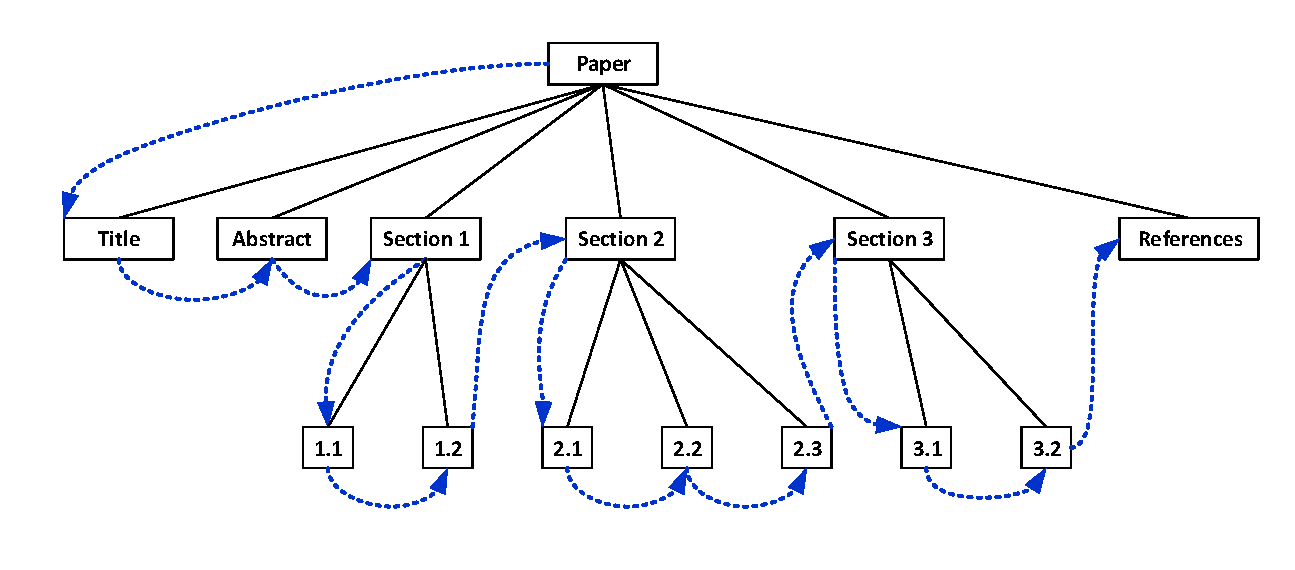
\includegraphics[width=\textwidth]{/TransversalOrderedTree.pdf}
					\caption{Preorder traversal of an ordered tree, where the children of each node are ordered from left to right.}
					\label{fig:TransversalOrderedTree}
				\end{figure}
				
So again, in this thesis the accessing order is exactly like a preorder traversal and there is a linear ordering of children so that we always know the recursive algorithms implemented for different task are done		
		
		\textbf{Quad Trees}\\
		
		A \textbf{quad tree} is an ordered tree in which each node has at most four children
		\begin{enumerate}
			\item Every node has at most four children.
			\item Each child node can be labeled as south-west(SW), south-east(SE), north-west(NW) or north-east(NE).
			\item The ordering of a node is implemented as SW$\rightarrow$SE$\rightarrow$NW$\rightarrow$NE. 
		\end{enumerate}
		A quad tree is termed to be \textbf{proper} if each node has either zero or four children.\\
		
		\textbf{A Recursive Quad Tree Definition}\\
		A recursive quad tree can be defined as a quad tree which
		\begin{itemize}
			\item is either empty
			\item consists of a node which is \textbf{root} and four further quad trees which are called as south-west(SW), south-east(SE), north-west(NW) or north-east(NE) subtrees. 
		\end{itemize}
		 
		 Figure \ref{fig:NodeQuadTree1} shows a representation of a node in a linked data structure for representing a quad tree.
		 		
		 \begin{figure}[h]
		 	\centering
		 	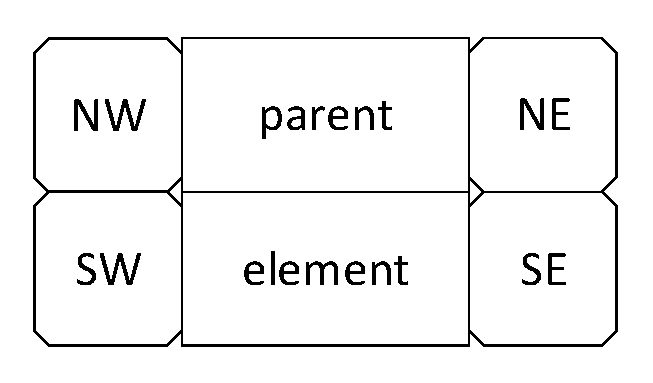
\includegraphics[width=0.33\textwidth]{/NodeQuadTree.pdf}
		 	\caption{A node in a linked data structure for representing a quad tree.}
		 	\label{fig:NodeQuadTree1}
		 \end{figure}

 \section{Main scheme of the implementation}
 
 To present the idea of main scheme which the work of this thesis is based upon an example of data structure and how the solution tree looks like is given in figure \ref{fig:QuadTreeRoot1}. The main reason here is that based on this visual element every aspect of the underlying refinement scheme can be observed. First, the root of this tree is the initial combination solution projected to a full grid. A total error after comparing the result to the normal full grid in the node will be evaluated and if it is higher than a predefined threshold then that node will be refined. Certainly for the root we require that it always gets refined. \\
 One should note that under the refinement, a node basically will be internal and produces four children namely SW,SE,NW,NE thus the naming quad tree. Basically a new node is the same as the initial node in that it will be produced with same level vector using a combination technique so it can be imagined exactly as another node of the tree which can also be refined if needed. Application to higher dimensions should seem straightforward after this.\\
 
 \begin{figure}[h]
	\centering
	    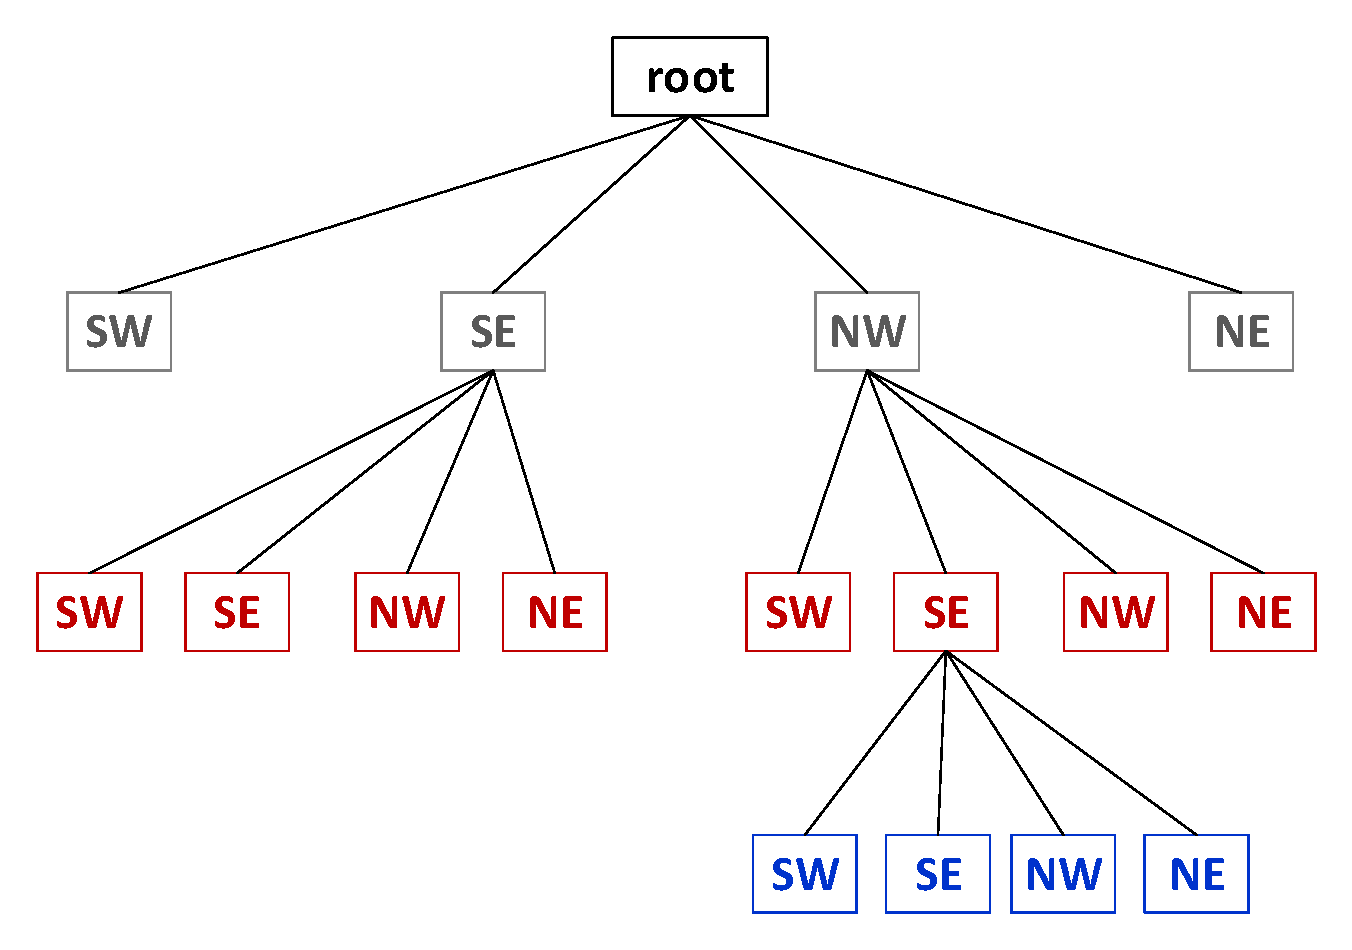
\includegraphics[width =0.66\textwidth]{/results/3/QuadTreeRoot.pdf}
	    %\vspace{3em}
		\centering
        \caption{Quad tree representation}
        \label{fig:QuadTreeRoot1}
\end{figure}

 Important discussion again was that we stick to the same pattern in our lower nodes. This can be seen exactly in the figure \ref{fig:Predef2}.
 
\begin{figure}[!ht]
	\centering
	    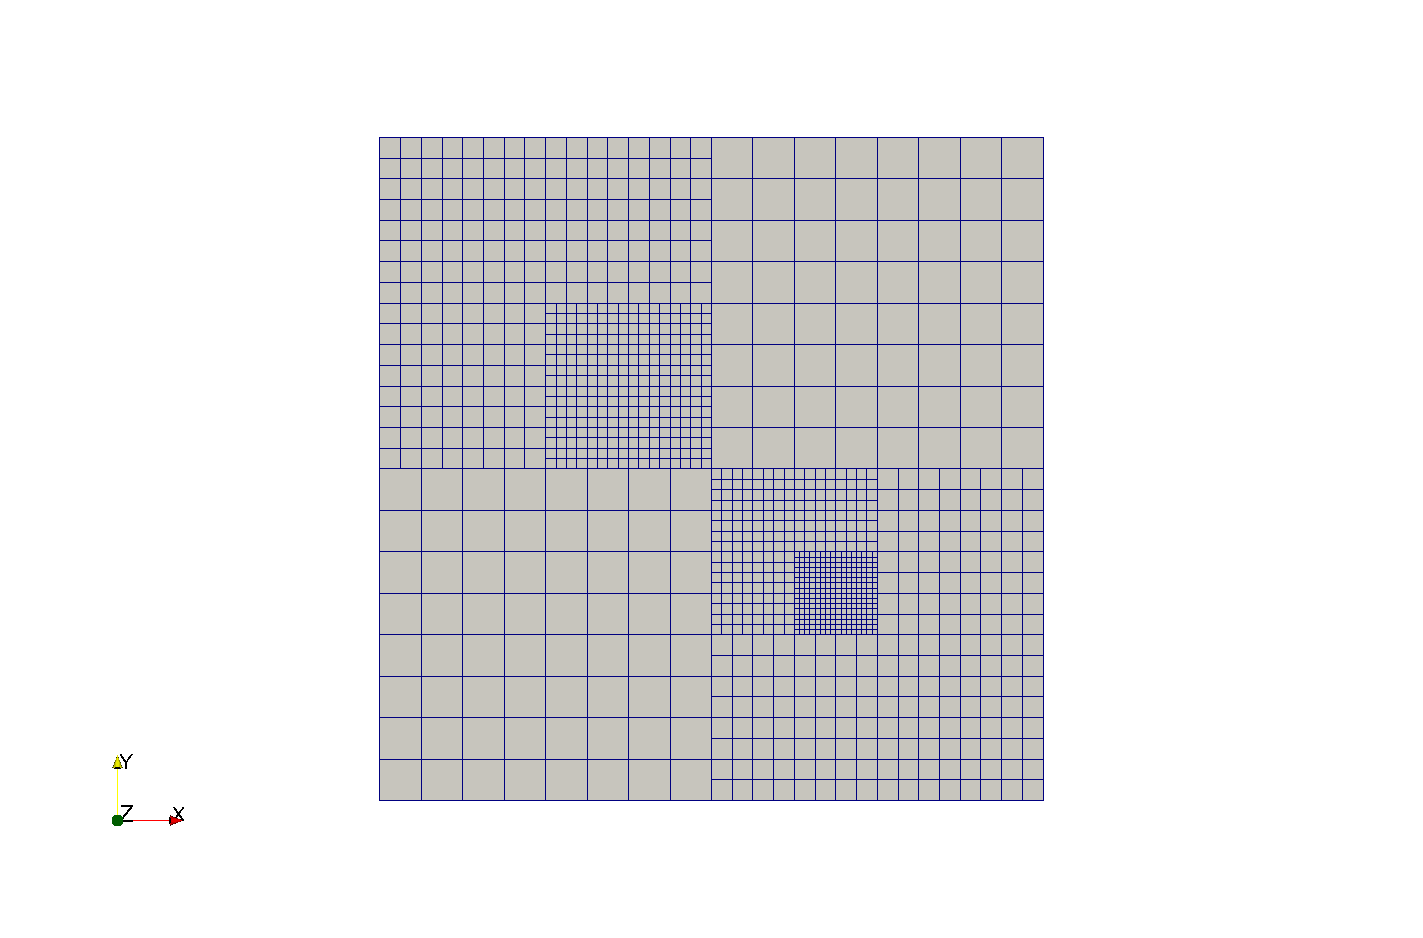
\includegraphics[width =\textwidth]{/results/3/predefined-refinement-vtk.png}
	    %\vspace{3em}
    \caption{Example of main scheme}
    \label{fig:Predef2}
\end{figure}
 


